 and how expanding a solution leads to symmetries (symmetric 
polynomials by today's verbage).
\begin{align*}
    \begin{array}{|c|cc|}
        \hline
        \times & x & -b \\
        \hline
        x & x^2 & {\color{blue} -bx}\\
        -a & {\color{blue} -ax} & {\color{red} ab} \\
    \hline
    \end{array}
    & \leadsto (x-a)(x-b)=x^2{\color{blue} -(a+b)x}{\color{red}+ab}
\end{align*}
We can flip the square along the diagonal like the transpose of a matrix 
and get the same product.  Thus a symmetry that moves the roots leave the 
resulting polynomial unchanged.  For cubics we get symmetries on a cube.
\begin{center}
    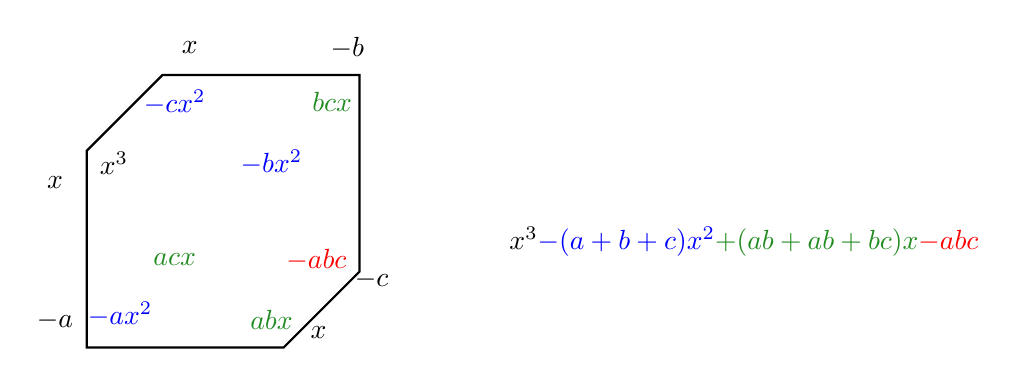
\begin{tikzpicture}
        \draw[thick] (-0.25,0.25,0.25)
            -- ++ (0,0,-2.5)
            -- ++ (2.5,0,0)
            -- ++ (0,-2.5,0)
            -- ++ (0,0,2.5)
            -- ++ (-2.5,0,0)
            -- cycle;
        \node (xx1) at (-0.75,-.25,0) {$x$};
        \node (xx2) at (0,0.5,-2.5) {$x$};
        \node (xx3) at (2.5,-2.25,-0.25) {$x$};
        \node (a) at (-0.75,-2,0) {$-a$};
        \node (b) at (2,0.5,-2.5) {$-b$};
        \node (c) at (2.5,-2.25,-2) {$-c$};

        \node (x3) at (0,0,0) {$x^3$};
        \node[blue] (ax2) at (0,-2,-0.2) {$-ax^2$};
        \node[blue] (bx2) at (2,0,0) {$-bx^2$};
        \node[blue] (cx2) at (0,0,-2) {$-cx^2$};
        \node[ForestGreen] (abx) at (2,-2,0) {$abx$};
        \node[ForestGreen] (acx) at (0,-2,-2) {$acx$};
        \node[ForestGreen] (bcx) at (2,0,-2) {$bcx$};
        \node[red] (abc) at (1.8,-2,-2) {$-abc$};

        \node at (8,-1,0) {$x^3{\color{blue}-(a+b+c)x^2}{\color{ForestGreen}+(ab+ab+bc)x}{\color{red}-abc}$};
    \end{tikzpicture}
\end{center}
Notice you can rotate or swap the three adjacent faces (permuting the three roots around) 
without interfering in the equation.  4th degree?  Explore symmetries on a hypercube.
\begin{center}
    \begin{tikzpicture}
        \draw[thick] (-4,0.5,0.5)
        -- ++ (0,0,-4.5)
        -- ++ (6.75,0,0)
        -- ++ (0,-3,0)
        -- ++ (0,0,4.5)
        -- ++ (-6.75,0,0)
        -- cycle;
        \node (xx4) at (-2,-3,0.5) {$x$};
        \node (d) at (2,-3,0.5) {$-d$};
        \node at (-2,0) {\begin{tikzpicture}
        \draw[thick] (-0.25,0.25,0.25)
            -- ++ (0,0,-2.5)
            -- ++ (2.5,0,0)
            -- ++ (0,-2.5,0)
            -- ++ (0,0,2.5)
            -- ++ (-2.5,0,0)
            -- cycle;
        \node (xx1) at (-0.75,-.25,0) {$x$};
        \node (xx2) at (0,0.5,-2.5) {$x$};
        % \node (xx3) at (2.5,-2.25,-0.25) {$x$};
        \node (a) at (-0.75,-2,0) {$-a$};
        \node (b) at (2,0.5,-2.5) {$-b$};
        % \node (c) at (2.5,-2.25,-2) {$-c$};

        \node (x3) at (0,0,0) {$x^4$};
        \node[blue] (ax2) at (0,-2,-0.2) {$-ax^3$};
        \node[blue] (bx2) at (2,0,0) {$-bx^3$};
        \node[blue] (cx2) at (0,0,-2) {$-cx^3$};
        \node[ForestGreen] (abx) at (2,-2,0) {$abx^2$};
        \node[ForestGreen] (acx) at (0,-2,-2) {$acx^2$};
        \node[ForestGreen] (bcx) at (2,0,-2) {$bcx^2$};
        \node[red] (abc) at (1.8,-2,-2) {$-abcx$};

        % \node at (8,-1,0) {$x^3{\color{blue}-(a+b+c)x^2}{\color{ForestGreen}+(ab+ab+bc)x}{\color{red}-abc}$};
        \end{tikzpicture}};
        \node at (2,0) {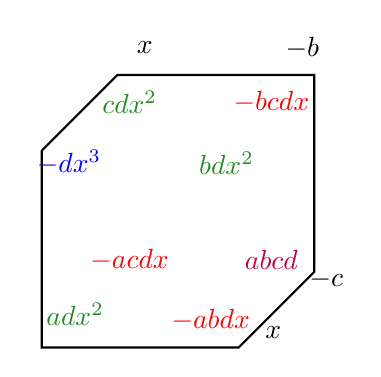
\begin{tikzpicture}
            \draw[thick] (-0.25,0.25,0.25)
                -- ++ (0,0,-2.5)
                -- ++ (2.5,0,0)
                -- ++ (0,-2.5,0)
                -- ++ (0,0,2.5)
                -- ++ (-2.5,0,0)
                -- cycle;
            % \node (xx1) at (-0.75,-.25,0) {$x$};
            \node (xx2) at (0,0.5,-2.5) {$x$};
            \node (xx3) at (2.5,-2.25,-0.25) {$x$};
            % \node (a) at (-0.75,-2,0) {$-a$};
            \node (b) at (2,0.5,-2.5) {$-b$};
            \node (c) at (2.5,-2.25,-2) {$-c$};
    
            \node[blue] (x3) at (0,0,0) {$-dx^3$};
            \node[ForestGreen] (ax2) at (0,-2,-0.2) {$adx^2$};
            \node[ForestGreen] (bx2) at (2,0,0) {$bdx^2$};
            \node[ForestGreen] (cx2) at (0,0,-2) {$cdx^2$};
            \node[red] (abx) at (1.8,-2,0) {$-abdx$};
            \node[red] (acx) at (0,-2,-2) {$-acdx$};
            \node[red] (bcx) at (1.8,0,-2) {$-bcdx$};
            \node[purple] (abc) at (1.8,-2,-2) {$abcd$};
    
            % \node at (8,-1,0) {$x^3{\color{blue}-(a+b+c)x^2}{\color{ForestGreen}+(ab+ab+bc)x}{\color{red}-abc}$};
            \end{tikzpicture}};
        \end{tikzpicture}
\end{center}
Which contracts to 
\begin{gather*}
    \begin{array}{|c|cc|}
        \hline 
         \times & x & -d \\
         \hline
        x^3 & x^4 & {\color{blue}-dx^3}\\
        -(a+b+c)x^2 & {\color{blue}-(a+b+c)x^3} & {\color{ForestGreen}(ad+bd+cd)x^2}\\
        +(ab+ac+bc)x^1 & {\color{ForestGreen}(ab+ac+bc)x^2} & {\color{red}-(abd+acd+bcd)x}\\
        -abc  & {\color{red}-abc x} & {\color{purple} abcd}\\
        \hline
    \end{array}\\
    x^4{\color{blue}-(a+b+c+d)x^3}
    {\color{ForestGreen}+(ab+ac+ad+bc+bd+cd)x^2}
    {\color{red}-(abc+abd+bcd)x}
    {\color{purple}+abcd}.
\end{gather*}
Lagrange witnessed a fluke.  You can gather the 4 roots as linear combinations
\begin{align*}
    s_{()} & = a+b+c+d\\
    s_{(12)(34)} & = a-b+c-d\\
    s_{(13)(24)} & = a-c+b-d\\
    s_{(14)(34)} & = a-d+c-b
\end{align*}
When solving a quartic, the term $s_{()}$ appears as the negative coefficient of 
$x^3$.  He then worked out how that because the remaining three are linear symmetric 
polynomials we can use them to write the other coefficients 
$(ab+ac+ad+bc+bd+cd)$, $(abc+abd+bcd)$, and $(abcd)$ as polynomials in 
the remaining $s$'s.  This means we have a single cubic polynomial which solves 
for the three missing numbers.  Having solved for all three $s$'s we use 
linear algebra to solve for the roots.
\begin{align*}
    \begin{bmatrix} 
        1 & 1 & 1 & 1\\
        1 & -1 & 1 & -1\\
        1 & 1 & -1 & -1\\
        1 & -1 & -1 & 1
    \end{bmatrix}
    \begin{bmatrix}
        a\\ b\\ c\\ d 
    \end{bmatrix}
    & = 
    \begin{bmatrix}
        s_{()}\\
        s_{(12)(34)}\\
        s_{(13)(24)}\\
        s_{(14)(32)}
    \end{bmatrix}
\end{align*}


